\documentclass{article}

\usepackage[T1]{fontenc}
\usepackage[utf8]{inputenc}
\usepackage[spanish]{babel}
\usepackage{graphicx}
\usepackage{microtype}
\usepackage{xcolor}
\usepackage{amsmath}
\usepackage{amssymb}
\usepackage{mathtools}
\usepackage{xfrac}
\usepackage{booktabs}
\usepackage{hyperref}
\usepackage{siunitx}

\newcommand{\todox}{\(\mathit{\color{red}x}\)}
\newcommand{\ham}{\large{\texttt{ham}}}
\newcommand{\spam}{\large{\texttt{spam}}}
\newcommand{\fo}{\(\mathbf{F_1}\)}

\interfootnotelinepenalty=10000

\title{Aprendizaje Automático \\ Trabajo Práctico 2 --- 4 en |}
\author{Martín Fixman \and Leandro Matayoshi \and Fernando Gasperi}
\date{Segundo Cuatrimestre de 2016}

\begin{document}
\maketitle

\newpage

\section{Introducción}

Este trabajo se propone explorar la técnica de Q Learning que permite aprender una tarea
sin necesidad de conocer ni $\delta$ (la función de transición) ni $r$ (la función de recompensa).
Analizaremos el caso concreto del juego 4 en línea para comprender cómo aprende y cómo afectan
al aprendizaje las diferentes variables que podemos controlar.

\section{Jugadores}

Modelamos el tablero y el 4 en línea de forma tal que fuera fácil simular juegos con distintos tipos de jugadores para
realizar las pruebas. Programamos 3 jugadores:
\begin{itemize}
  \item Q Learning
  \item Random
  \item Minimax
\end{itemize}
El jugador Minimax tiene un horizonte de 5 jugadas. Si no alcanza una posición final mirando 5 jugadas
hacia adelante devuelve medio punto para el jugador que más cerca esté de alcanzar 4 en línea verticalmente.
No se nos ocurrió una forma rápida de evaluar las posiciones del juego sin recorrer todo el tablero y calcular
por fuerza bruta quién se encuentra a menos movimientos de conseguir 4 en línea. Considerar sólo las oportunidades
verticales nos pareció una alternativa razonable entre el cálculo completo y la ausencia de evaluación.
El jugador Q Learning tiene varios parámetros que permiten ajustarlo:
\begin{itemize}
  \item $\epsilon$ es la probabilidad con la cual elige una acción al azar. En
    cada turno elige con probabilidad $\epsilon$ tomar una acción al azar entre
    las disponibles o tomar alguna de las que maximiza Q para el estado actual.
  \item $\alpha$ es la tasa de aprendizaje, el peso que le damos a lo aprendido
    con la nueva acción.
  \item $\gamma$ es la constante que determina el valor relativo de las
    recompensas futuras.
  \item el valor inicial de los elementos $Q_{i, j}$.
\end{itemize}
Las experimentaciones que realizaremos pretenden analizar cómo impactan estos
parámetros en el aprendizaje del jugador. Además nos interesa ver el efecto de
cuestiones externas al algoritmo como si aprende jugando sólo con un color (lo
cual decide quién comienza las partidas), con qué jugador aprende, etc.



\section{Experimentación}

\subsection{Performance against Minimax}

Durante el TP se desarrolló una implementación de MinimaxPlayer que obtiene muy buenos resultados.
Utiliza una ventana de 3 movimientos a futuro, premiando los escenarios ganadores con un valor de 1,
castigando los escenarios perdedores con -1 y devolviendo 0 para los escenarios en donde la ventana alcanza
un valor de 0 y ningún jugador ha ganado o perdido.

Dicha implementación fue testeada contra un jugador random alcanzando un niveles de efectividad muy altos.
Debido a las características recursivas del algoritmo el algoritmo toma un tiempo no despreciable en ejecutarse,
por lo que experimentamos hasta una cantidad de juegos N con un valor máximo de 100.000

A continuación se incluye una tabla en donde mostramos la efectividad de un QLearn Player compitiendo contra
un Minimax player para distinta cantidad de juegos N.

Los parámetros del QLearn Player fueron fijados con los siguientes valores:
$\epsilon$ = 0.2, $\alpha$ = 0.3, $\gamma$ = 0.9

Los resultados están expresados en función de la cantidad de victorias del jugador QLearn sobre el total de partidos
jugados

~

\begin{center}
\begin{tabular}{c c}
	\toprule
	\textbf{\#Games} & \textbf{QLearn victories} \\
	\midrule
	0 & 0.01 \\
	1000 & 0.013 \\
	5000 & 0.0136 \\
	10000 & 0.0121 \\
	20000 & 0.01205 \\
	40000 & 0.012775 \\
	100000 & 0.0117 \\
	\bottomrule
\end{tabular}
\end{center}

~

Según los resultados podemos concluir que la cantidad de partidos jugados no son suficientes como para que el
algoritmo de QLearn desarrolle una política $\pi$ efectiva. Por el contrario, la ventana de valor 3
le es suficiente al Minimax player para poder anticipar y dirigir sus movimientos a escenarios ganadores y poder
evitar los perdedores.


\subsection{Tasa de aprendizaje}

A continuación incluimos los resultados de los experimentos en donde comparamos la forma en que el
QLearn player aprende a jugar contra distintos tipos de jugadores.

Realizamos 3 corridas diferentes, en donde variamos el rol del QLearn en el juego: Jugador
que realiza el primer movimiento, que mueve segundo o alternando los turnos de inicio.

Los parámetros del QLearn Player fueron fijados con los siguientes valores:
$\epsilon$ = 0.2, $\alpha$ = 0.3, $\gamma$ = 0.9

\begin{figure}[H]
	\centerline{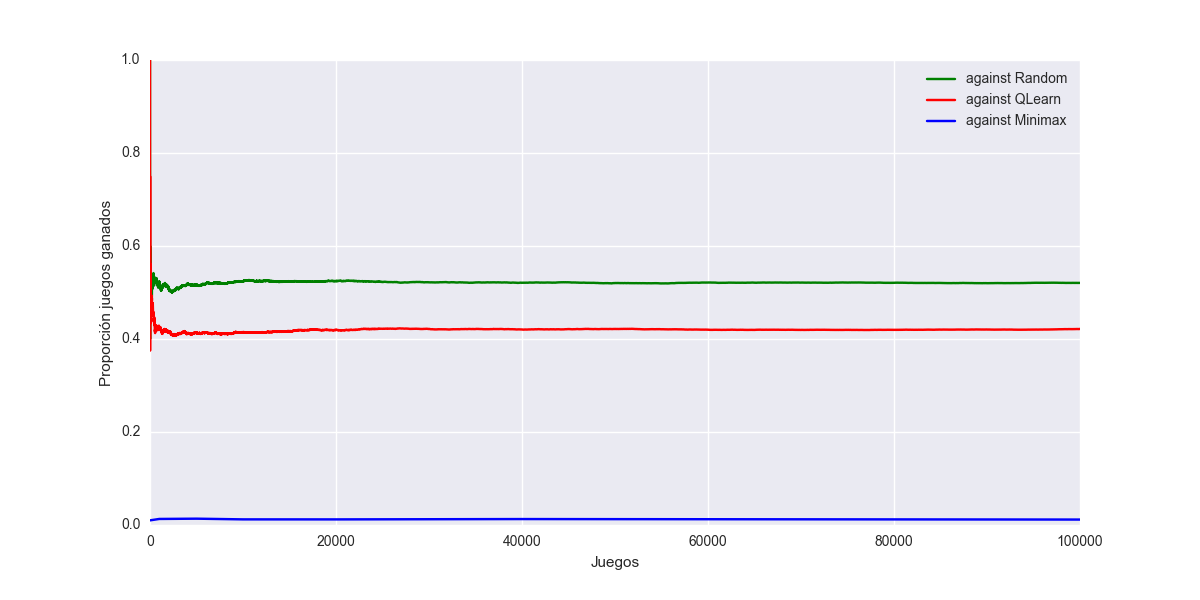
\includegraphics[width=1.3\textwidth]{figures/learning_rate_as_second_player.png}}
	\caption{Porcentaje de victorias como jugador que mueve segundo}
\end{figure}

\begin{figure}[H]
	\centerline{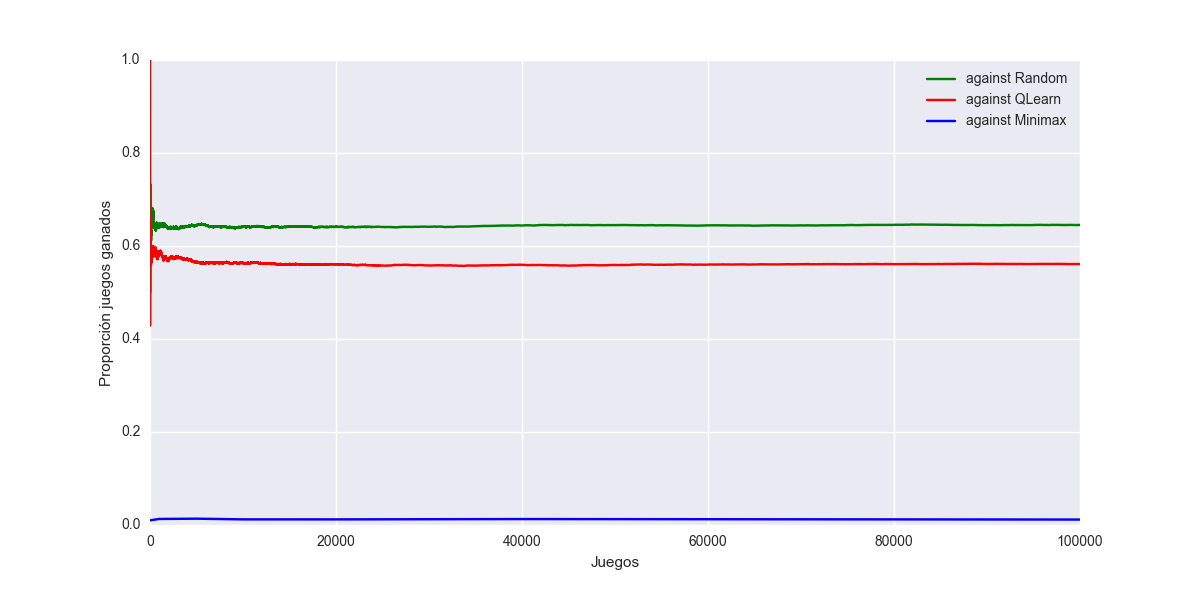
\includegraphics[width=1.3\textwidth]{figures/learning_rate_as_first_player.png}}
	\caption{Porcentaje de victorias como jugador que mueve primero}
\end{figure}

\begin{figure}[H]
	\centerline{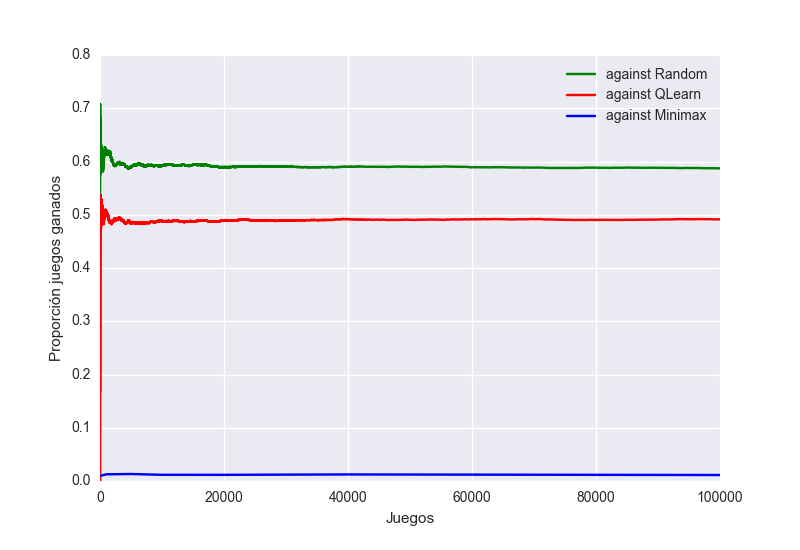
\includegraphics[width=1.3\textwidth]{figures/learning_rate_rotating_turns.png}}
	\caption{Porcentaje de victorias alternando los turnos de inicio}
\end{figure}

En los 3 casos observamos malos resultados. El porcentaje de victorias permanece constante para esa cantidad
de juegos, lo que da un indicio de que el algoritmo no obtiene mejoras inmediatas en su aprendizaje según
el tipo de jugador ni dependiendo de si empieza primero o segundo (aunque obtiene más victorias cuando
mueve primero).


\section{Conclusiones}

\end{document}
